%!TEX program = xelatex

% Name           : mpimg-beamer-minimal.sty
% Author         : Martin Ballaschk (ballaschk@molgen.mpg.de)
%                  based on a theme by Benjamin Weiss (benjamin.weiss@kreatiefton.de)
% Version        : 0.1
% Created on     : 07.03.2021
% Copyright      : Copyright (c) 2013 by Benjamin Weiss. All rights reserved.
% License        : This file may be distributed and/or modified under the
%                  GNU Public License.
% Description    : MPIMG beamer theme minimal example.

\documentclass[compress%
,aspectratio=169% uncomment for 3:4 slides
]{beamer}

\usepackage[english]{babel}
\usepackage{tikz}
\usepackage{listings}
\usepackage{tabularx}
\usepackage{booktabs}
\usepackage{fontspec}
\usepackage{hyperref}
\usepackage{siunitx}
\usepackage[super]{nth}
\setmonofont{Roboto Mono}[Scale=MatchLowercase] % select a suitable monospaced font
% https://www.overleaf.com/learn/latex/Questions/Which_OTF_or_TTF_fonts_are_supported_via_fontspec%3F#Monospaced_fonts

\usetheme{mpimg}
\definecolor{mygray}{rgb}{0.9,0.9,0.9}
%%%%%%%%%%%%%%%%%%%%%%%%%%%%
% python highlighting
% https://tex.stackexchange.com/questions/235783/listings-recognize-numbers-and-1e-3

% \definecolor{halfgray}{gray}{0.55}
% \definecolor{ipython_frame}{RGB}{207, 207, 207}
% \definecolor{ipython_bg}{RGB}{247, 247, 247}
% \definecolor{ipython_red}{RGB}{186, 33, 33}
% \definecolor{ipython_green}{RGB}{0, 128, 0}
% \definecolor{ipython_cyan}{RGB}{64, 128, 128}
% \definecolor{ipython_purple}{RGB}{170, 34, 255}
\definecolor{maroon}{cmyk}{0, 0.87, 0.68, 0.32}
\definecolor{halfgray}{gray}{0.55}
\definecolor{ipython_frame}{RGB}{207, 207, 207}
\definecolor{ipython_bg}{RGB}{247, 247, 247}
\definecolor{ipython_red}{RGB}{186, 33, 33}
\definecolor{ipython_green}{RGB}{0, 128, 0}
\definecolor{ipython_cyan}{RGB}{64, 128, 128}
\definecolor{ipython_purple}{RGB}{170, 34, 255}
\definecolor{mpgGreyLight_bg}{RGB}{238,238,238} %(R=238 G=238 B=238)

\usepackage{listings}
\lstset{
    % escapeinside={(*@}{@*)},
    breaklines=true,
    %
    extendedchars=true,
    literate=
    {á}{{\'a}}1 {é}{{\'e}}1 {í}{{\'i}}1 {ó}{{\'o}}1 {ú}{{\'u}}1
    {Á}{{\'A}}1 {É}{{\'E}}1 {Í}{{\'I}}1 {Ó}{{\'O}}1 {Ú}{{\'U}}1
    {à}{{\`a}}1 {è}{{\`e}}1 {ì}{{\`i}}1 {ò}{{\`o}}1 {ù}{{\`u}}1
    {À}{{\`A}}1 {È}{{\'E}}1 {Ì}{{\`I}}1 {Ò}{{\`O}}1 {Ù}{{\`U}}1
    {ä}{{\"a}}1 {ë}{{\"e}}1 {ï}{{\"i}}1 {ö}{{\"o}}1 {ü}{{\"u}}1
    {Ä}{{\"A}}1 {Ë}{{\"E}}1 {Ï}{{\"I}}1 {Ö}{{\"O}}1 {Ü}{{\"U}}1
    {â}{{\^a}}1 {ê}{{\^e}}1 {î}{{\^i}}1 {ô}{{\^o}}1 {û}{{\^u}}1
    {Â}{{\^A}}1 {Ê}{{\^E}}1 {Î}{{\^I}}1 {Ô}{{\^O}}1 {Û}{{\^U}}1
    {œ}{{\oe}}1 {Œ}{{\OE}}1 {æ}{{\ae}}1 {Æ}{{\AE}}1 {ß}{{\ss}}1
    {ç}{{\c c}}1 {Ç}{{\c C}}1 {ø}{{\o}}1 {å}{{\r a}}1 {Å}{{\r A}}1
    {€}{{\EUR}}1 {£}{{\pounds}}1
}

%%
%% Python definition (c) 1998 Michael Weber
%% Additional definitions (2013) Alexis Dimitriadis
%% modified by me (should not have empty lines)
%%
\lstdefinelanguage{iPython}{
    morekeywords={access,and,break,class,continue,def,del,elif,else,except,exec,finally,for,from,global,if,import,in,is,lambda,not,or,pass,print,raise,return,try,while},%
    %
    % Built-ins
    morekeywords=[2]{abs,all,any,as,basestring,bin,bool,bytearray,callable,chr,classmethod,cmp,compile,complex,delattr,dict,dir,divmod,enumerate,eval,execfile,filter,float,format,frozenset,getattr,globals,hasattr,hash,help,hex,id,input,int,isinstance,issubclass,iter,len,list,locals,long,map,max,memoryview,min,next,object,oct,open,ord,pow,property,range,raw_input,reduce,reload,repr,reversed,round,set,setattr,slice,sorted,staticmethod,str,sum,super,tuple,type,unichr,unicode,vars,xrange,zip,apply,buffer,coerce,intern,NoneType,array, show, imshow, convolve, square, sqrt, dot, DataFrame, Series, Dog, add_tricks, describe, imread, shape, add_trick, append, read, splitlines, write, while, with, to_csv, savetxt, genfromtxt, read_csv},%
    %
    sensitive=true,%
    morecomment=[l]\#,%
    morecomment=[l]Out:,
    morestring=[b]',%
    morestring=[b]",%
    %
    morestring=[s]{'''}{'''},% used for documentation text (mulitiline strings)
    morestring=[s]{"""}{"""},% added by Philipp Matthias Hahn
    %
    morestring=[s]{r'}{'},% `raw' strings
    morestring=[s]{r"}{"},%
    morestring=[s]{r'''}{'''},%
    morestring=[s]{r"""}{"""},%
    morestring=[s]{u'}{'},% unicode strings
    morestring=[s]{u"}{"},%
    morestring=[s]{u'''}{'''},%
    morestring=[s]{u"""}{"""},%
    %
    % {replace}{replacement}{lenght of replace}
    % *{-}{-}{1} will not replace in comments and so on
    literate=
    {á}{{\'a}}1 {é}{{\'e}}1 {í}{{\'i}}1 {ó}{{\'o}}1 {ú}{{\'u}}1
    {Á}{{\'A}}1 {É}{{\'E}}1 {Í}{{\'I}}1 {Ó}{{\'O}}1 {Ú}{{\'U}}1
    {à}{{\`a}}1 {è}{{\`e}}1 {ì}{{\`i}}1 {ò}{{\`o}}1 {ù}{{\`u}}1
    {À}{{\`A}}1 {È}{{\'E}}1 {Ì}{{\`I}}1 {Ò}{{\`O}}1 {Ù}{{\`U}}1
    {ä}{{\"a}}1 {ë}{{\"e}}1 {ï}{{\"i}}1 {ö}{{\"o}}1 {ü}{{\"u}}1
    {Ä}{{\"A}}1 {Ë}{{\"E}}1 {Ï}{{\"I}}1 {Ö}{{\"O}}1 {Ü}{{\"U}}1
    {â}{{\^a}}1 {ê}{{\^e}}1 {î}{{\^i}}1 {ô}{{\^o}}1 {û}{{\^u}}1
    {Â}{{\^A}}1 {Ê}{{\^E}}1 {Î}{{\^I}}1 {Ô}{{\^O}}1 {Û}{{\^U}}1
    {œ}{{\oe}}1 {Œ}{{\OE}}1 {æ}{{\ae}}1 {Æ}{{\AE}}1 {ß}{{\ss}}1
    {ç}{{\c c}}1 {Ç}{{\c C}}1 {ø}{{\o}}1 {å}{{\r a}}1 {Å}{{\r A}}1
    {€}{{\EUR}}1 {£}{{\pounds}}1,
    %
    literate=
    *{+}{{{\color{ipython_purple}+}}}1
    {-}{{{\color{ipython_purple}-}}}1
    {*}{{{\color{ipython_purple}$^\ast$}}}1
    {/}{{{\color{ipython_purple}/}}}1
    {^}{{{\color{ipython_purple}\^{}}}}1
    {?}{{{\color{ipython_purple}?}}}1
    {!}{{{\color{ipython_purple}!}}}1
    {\%}{{{\color{ipython_purple}\%}}}1
    {<}{{{\color{ipython_purple}<}}}1
    {>}{{{\color{ipython_purple}>}}}1
    {|}{{{\color{ipython_purple}|}}}1
    {\&}{{{\color{ipython_purple}\&}}}1
    {~}{{{\color{ipython_purple}~}}}1
    %
    {==}{{{\color{ipython_purple}==}}}2
    {<=}{{{\color{ipython_purple}<=}}}2
    {>=}{{{\color{ipython_purple}>=}}}2
    %
    {>>>}{{{\color{ipython_cyan}>>>}}}3
    %
    {+=}{{{+=}}}2
    {-=}{{{-=}}}2
    {*=}{{{$^\ast$=}}}2
    {/=}{{{/=}}}2,
    %
%   identifierstyle=\color{red}\ttfamily,
    commentstyle=\color{ipython_cyan}\ttfamily,
    stringstyle=\color{ipython_red}\ttfamily,
    keepspaces=true,
    showspaces=false,
    showstringspaces=false,
    %
    rulecolor=\color{ipython_frame},
    frame=single,
    frameround={t}{t}{t}{t},
    framexleftmargin=6mm,
    numbers=left,
    numberstyle=\tiny\color{halfgray},
    %
    %
    backgroundcolor=\color{ipython_bg},
    % backgroundcolor=\color{mpgGreyLight_bg},
    %   extendedchars=true,
    basicstyle=\scriptsize\ttfamily,
    keywordstyle=\color{ipython_green}\ttfamily,
    % escapechar=\¢,
    escapechar={|}
    % escapebegin=\color{ipython_green}
}
%%%%%%%%%%%%%%%%%%%%%%%%%%%%%%%%5


% For nice inline code
\usepackage{xpatch}
\usepackage{xcolor}
\usepackage{realboxes}


\lstset{
  language=iPython
  }
% \lstset{language=Python, style = colored}

\makeatletter
\xpretocmd\lstinline{\Colorbox{mygray}\bgroup\appto\lst@DeInit{\egroup}}{}{}
\makeatother

\newcommand{\code}{\lstinline}

\title{Python Basics}
\subtitle{Scripting Imaging Workshop}
\author{Clemens Kohl}
\institute{Max Planck Institute for Molecular Genetics}
\date{25.09.2023}

\begin{document}

\maketitle

% \section*{Outline}
\begin{frame}
	\frametitle{Outline}
	\tableofcontents[hideallsubsections]
\end{frame}

\setbeamertemplate{caption}{\raggedright\insertcaption\par}
\begin{frame}{Jupyter Notebook}
\begin{columns}
    \column{0.5\linewidth}
    \begin{itemize}
    \item Open Jupyter Notebook from Link
    \item File > "Save a Copy in Drive"
    \item Execute Cells with "Ctrl + Enter" or "Shift + Enter"
\end{itemize}
    \column{0.4\linewidth}
    \begin{figure}
    \centering
    
\includegraphics[width = 0.7\linewidth]{img/link.png}
    \caption{\alert{\url{www.tinyurl.com/sva6zv98}}}
\end{figure}
\end{columns}
\end{frame}


\begin{frame}{Get the slides (or don't)}

You can download the slides (and the code to generate them) from github:
    \begin{figure}
    \centering
    
\includegraphics[width = 0.3\linewidth]{img/github.png}
    \caption{\alert{\url{www.github.com/ClemensKohl/python_nanocourse}}}
    \end{figure}
    
\end{frame}
\setbeamertemplate{caption}[default]


\section{Data Types}

\begin{frame}[fragile]{Data Types}

    \begin{itemize}
        \item What are data types and why should you care?
    \end{itemize}
    % Example:
\begin{lstlisting}[language=iPython]
2 + 3 = ?
"hello" + "world" = ?
True + False = ?
True + 1 = ?
["version"] + [2] = ?
\end{lstlisting}
    
\end{frame}

\begin{frame}[fragile]{Data Types}

    \begin{itemize}
        \item What are data types and why should you care?
    \end{itemize}
    % Example:
\begin{lstlisting}
>>> 2 + 3
Out: 5
>>> "hello" + "world"
Out: "helloworld"
>>> True + False
Out: 1
>>> True + 1
Out: 2
>>> ["version"] + [2]
Out: ['version', 2]
\end{lstlisting}
Different types can do different things!
\end{frame}

\begin{frame}[fragile]{Data Types}

Built in Python data types:
\begin{table}
\tiny
\setlength\fboxsep{1.5pt} % Controls the padding around the code boxes.
\begin{tabularx}{\textwidth}{llX}
    \toprule
    \textbf{Data Type}  & \textbf{Name}  & \textbf{Example}   \\
    \midrule
    Numbers         &  \code|int|,  \code|float|,  \code|complex| & \code|1234|, \code|3.1415|, \code|3+4j| \\
    Text            &  \code|str|      & \code|'spam'|, \code|"Bob's"|    \\
    Sequences       &  \code|list|,  \code|tuple|,  \code|range|  & \code|[1, 'two', 3.0]|,  \code|("a", "b", "c")|,  \code|range(3)| \\
    Mapping Type    &  \code|dict|     & \code|\{'food': 'spam', 'taste': 'yum'\}|  \\
    Sets            &  \code|set|      & \code|set('abc')|, \code|\{'a', 'b', 'c'\}| \\           
    Boolean         &  \code|bool|     & \code|True|, \code|False|  \\
    None Types      & \code|NoneType|  & \code|None| \\
    \bottomrule
\end{tabularx}
\end{table}

You can get the data type of an object by using \lstinline|type()|:
\begin{lstlisting}
>>> type("word")
Out: <class 'str'>
\end{lstlisting}

\end{frame}


\begin{frame}[fragile]{Python Lists}

\begin{itemize}
    \item Python lists can contain elements of any type.
    \item Python lists are 1 dimensional (they can be nested though).
    \item Element-wise operations require a loop.
\end{itemize}
\begin{lstlisting}
x_list = ["a", 1, 2.3, True, False, 3]
\end{lstlisting}
\nth{2} to \nth{4} element of the list:
\begin{lstlisting}
>>> x_list[1:4]
Out: [1, 2.3, True]
\end{lstlisting}
\begin{alertblock}{Note}
Python is 0 indexed! The slicing start point is inclusive and the end point is exclusive.
\end{alertblock}
\end{frame}

\begin{frame}[fragile]{dictionaries}
\vspace{-0.3cm}
\begin{itemize}
    \item Dictionaries are "key" - "value" pairs. 
    \item Keys need to be unique, values can be anything.
    \item dictionaries are created with \code|{}| or \code{dict()}
\end{itemize}
\vspace{0.1cm}

\begin{columns}
    \column{0.3\linewidth}
\begin{lstlisting}
microscope = {
  "brand": "Zeiss",
  "model": "LSM 980",
  "year": 2020,
  "price": 999999
}
\end{lstlisting}

    \column{0.6\linewidth}
\footnotesize Access elements, add new ones or change existing ones:
\begin{lstlisting}
>>>  print(microscope["brand"])
Out: "Zeiss"
>>> microscope["broken"] = True
>>> microscope["price"] = 200
\end{lstlisting}
\end{columns}
Keys and values are accessed through \code{dict.keys()} and \code{dict.values()}
\begin{lstlisting}
>>> microscope.keys()
Out: dict_keys(['brand', 'model', 'year', 'price', 'broken'])
>>> microscope.values()
Out: dict_values(['Zeiss', 'LSM 980', 2020, 200, True])
\end{lstlisting}

\end{frame}

\begin{frame}[fragile]{Numpy Arrays}
    
\begin{itemize}
    \item Numpy arrays contain elements of similar type.
    \item Numpy arrays are N-dimensional.
    \item Allow for element-wise operations.
    \item Usually more efficient.
\end{itemize}

\begin{lstlisting}
import numpy as np
x = np.array([[1,2],        # 2-dimensional
              [3,4],
              [5,6]])           

y = np.array([[[1,2,3],     # 3-dimensional
               [4,5,6]],          
              [[7,8,9],
               [9,8,7]]])
\end{lstlisting}
    
\end{frame}

\section{Python as a calculator}

% https://docs.python.org/3/tutorial/introduction.html#using-python-as-a-calculator
\begin{frame}[fragile]{Basic Math}
    \begin{itemize}
        \item Basic Math operations:
    \end{itemize}

\begin{lstlisting}
a = 1+2-10      # add/subtracting numbers up
b = (7*4)/2     # multiplication and division
c = a**2        # raise to the power of x
\end{lstlisting}

    \begin{itemize}
        \item Results can be either "integers" or "floats":
    \end{itemize}

\begin{lstlisting}
>>> 50 - 5*6
Out: 20
>>> 17 / 3
Out: 5.666666666666667
\end{lstlisting}

\begin{itemize}
    \item Division always returns a float!
\end{itemize}
\end{frame}


\begin{frame}[fragile]{More Math operations}

\begin{itemize}
    \item Floor division and the modulo operation:
\end{itemize}
    \begin{lstlisting}
>>> 17 // 3  # floor division discards the fractional part
Out: 5

>>> 17 % 3  # the % operator returns the remainder of the division
Out: 2
    \end{lstlisting}
\end{frame}


\begin{frame}[fragile]{Precision: Integers and Floats}

\begin{itemize}
    \item Computers can only calculate with limited precision.
    \item This can lead to unexpected behaviour:
\begin{lstlisting}
>>> 0.1 + 0.2
Out: 0.30000000000000004
>>> 0.1 + 0.2 == 0.3
Out: False
\end{lstlisting}
\end{itemize}

\begin{itemize}
    \item \textbf{Explanation:} 0.1 in binary is a infinitely repeating number similar to ⅓ in decimal base.
    \item This phenomenon called \textit{Representation Error} is very common and needs to be taken into account.
\begin{lstlisting}
>>> format(0.1, ".20g")
Out: '0.10000000000000000555'
\end{lstlisting}    
\end{itemize}

\end{frame}

\begin{frame}[fragile]{Comparing Floats}
    
\textbf{Solution:}
\begin{lstlisting}
>>> import math
>>> math.isclose(0.1 + 0.2, 0.3)
Out: True

>>> import numpy as np
>>> np.allclose([1e10, 1e-8], [1.00001e10, 1e-9])
Out: True
>>> np.isclose([1e10, 1e-7], [1.00001e10, 1e-8])
Out: array([ True, False])
\end{lstlisting}

\begin{itemize}
    \item Tolerances of the functions can be set as needed.
    \alert{\item \textbf{Don't compare floats directly!}}
\end{itemize}


\end{frame}

\begin{frame}[fragile]{Basic NumPy Operations}
\begin{lstlisting}
img = np.random.randint(0, 255, size=(500,500,3)) # random matrix

img[i,:,:] = img[j,:]     # set the values of row i with values from row j
img[:,i] = 100          # set all values in column i to 100
img[:100, :50, :].sum()     # the sum of the values of the first 100 rows and 50 columns
img[50:100, 50:100, :]      # rows 50-100, columns 50-100 (100th not included)
img[i].mean()           # average of row i
img[:,-1]               # last column
img[-2,:]               # second to last row

\end{lstlisting}
\end{frame}

\begin{frame}[fragile]{Vectorization with numpy}
% \textbf{Note:} The order of channels is RGB for matplotlib and PIL, but BGR for cv2!

% Continuing with the starry night image:
    \begin{lstlisting}
# Average RGB value.
mimg = img.mean(axis=2)
plt.imshow(mimg, cmap='gray')
plt.show()

# show max value per channel
plt.imshow(img.max(axis = 2), cmap='gray')
plt.show()

print(img.max())
print(img.min())
    \end{lstlisting}

\begin{alertblock}{Channel Order}
The order of channels is RGB for matplotlib and PIL, but BGR for cv2!
\end{alertblock}

\end{frame}

\begin{frame}[fragile]{More vectorization}
\begin{lstlisting}
a = np.random.randint(0, 255, size=100)
b = np.random.randint(0, 255, size=100)

c = a - b           # element-wise subtraction.
a_transpose = a.T   # transpose

# index of max value
np.argmax(a)
np.where(a == np.max(a))
\end{lstlisting}

\end{frame}

\begin{frame}[fragile]{Vector and matrix multiplication}
    
\begin{columns}
    \column{0.6\linewidth}
\begin{lstlisting}
# scalar projection of a onto b.
a1_length = np.dot(a,b)/np.linalg.norm(b)
\end{lstlisting}
\column{0.3\linewidth}
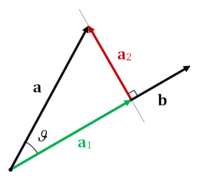
\includegraphics[width=0.8\linewidth]{img/scalar_projection.png}
\end{columns}

\begin{lstlisting}
# multiply two 2D matrices
A = np.random.randint(0, 255, size=(500,250)) 
B = np.random.randint(0, 255, size=(500,250))
AxB = np.dot(A, B.T)

# multiply two 3D matrices
# matmul assumes 2D matrices in last two indices!
img = img.reshape(3, img.shape[0], img.shape[1])
mult_img = np.matmul(img, img.transpose((0,2,1)))
\end{lstlisting}
% \textbf{Note:} The order of channels is RGB for matplotlib and PIL, but BGR for cv2!
\end{frame}

\begin{frame}{Tensor contraction}
\begin{itemize}
    \item Generalization of Matrix Multiplication for >2 dimensions.
    \item If you are mad enough to do this, you clearly don't need me.
    \item Look into \code{torch.tensordot()} from \code{pytorch}.
\end{itemize}
The easy to understand formula tensordot computes:
$$r_{i_0,...,i_{m-d}, i_d,...,i_n} = \sum_{k_0,...,k_{d-1}} a_{i_0,...,i_{m-d},k_0,...,k_{d-1}} \times b_{k_0,...,k_{d-1}, i_d,...,i_n}$$
\end{frame}
\section{Loops and conditionals}



\begin{frame}[fragile]{if clauses}
\begin{itemize}
    \item Executes a set of statements if a condition is true.
    \item It can have zero or more \code|elif| (else if) statements and/or an optional single \code|else| statement.
\end{itemize}

\begin{lstlisting}
a = 200
b = 33
if b > a:
  print("b is greater than a")
elif a == b:
  print("a and b are equal")
else:
  print("a is greater than b")
\end{lstlisting}
\alert{Wherever possible, avoid nested conditions!}
\end{frame}




\begin{frame}[fragile]{for loops}

\begin{itemize}
    \item A for loop iterates over a sequence (called iterator, e.g. a list, tuple, dictionary, ...).
    \item Technically, the iterator must have a \lstinline{__iter__()} and \lstinline{__next__()} methods.
    \item Within the loop we can execute a set of statements.
\end{itemize}

Simple example:
\begin{lstlisting}
fruits = ["apple", "banana", "cherry"]

for x in fruits:
    print(x)
    if x == "banana":
        print("I don't like banana.")
\end{lstlisting}

\end{frame}

\begin{frame}[fragile]{continue and break}

\begin{itemize}
    \item The \code|continue| statement skips the current iteration.
    \item The \code|break| statement exits the the loop.
\end{itemize}

Examples:
\begin{lstlisting}
for i in range(1,10):
    if i == 5:
        continue
    print("Number", i)

for i in range(1,10):
    if i == 5:
        break
    print("Number", i)
\end{lstlisting}

\end{frame}

\begin{frame}[fragile]{Loop tips}
\begin{itemize}
\small
    \item Pre-allocate the memory for the output of a loop. 
    \item If possible \alert{do not append to a list} in each iteration.
\begin{lstlisting}
results = [None] * 1000         # Make a list of 1000 None's.
for i in range(1000):
    is_even = (i % 2) == 0
    results[i] = is_even        # Save result in spot in list.
\end{lstlisting}
\end{itemize}
\end{frame}

\begin{frame}[fragile]{Loop tips - 2}
\begin{itemize}
    \item use \code|enumerate()| and \code|zip()|
    
\begin{lstlisting}
nums = [1, 2, 3]
letters = ["a", "b", "c"]

for idx, val in enumerate(letters):     # get the index and value.
    print(idx, val)

for val1, val2 in zip(nums, letters):   # Loop over two lists.
    print(val1, val2)
\end{lstlisting}

    \item If you can, \alert{avoid for loops!}
    \item Use built-in or numpy functions instead.
\end{itemize}

\end{frame}




\begin{frame}[fragile]{List comprehension}
    \begin{itemize}
        \item Shorter syntax than for loop.
        \item No need to preallocate memory.
        \item Often faster than for loops.
        \item Street cred. More "pythonic".
    \end{itemize}
    
\begin{figure}
    \centering
    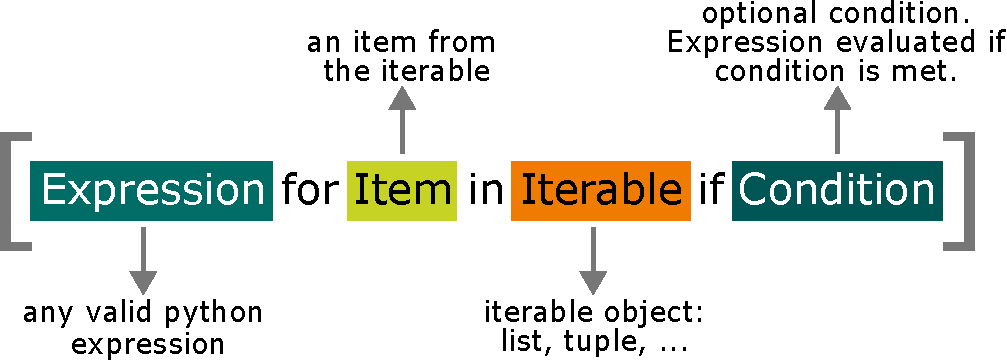
\includegraphics[width=0.6\linewidth]{img/list_comprehension.pdf}
\end{figure}
\end{frame}

\begin{frame}[fragile]{List comprehension - Example}
\begin{figure}
    \centering
    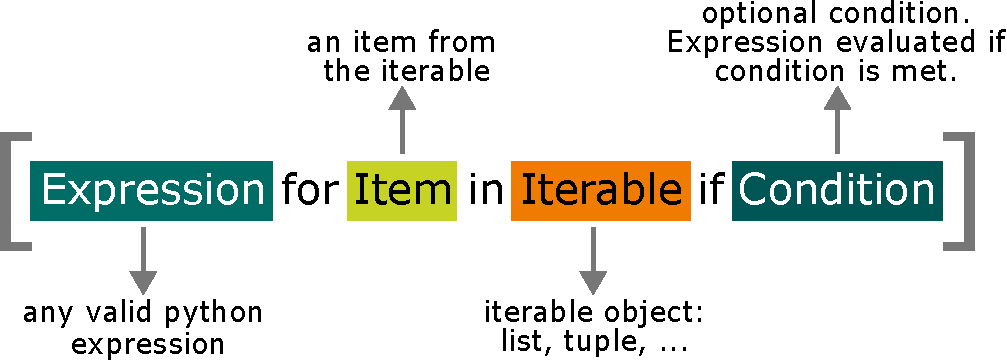
\includegraphics[width=0.6\linewidth]{img/list_comprehension.pdf}
\end{figure}

with for loop:
\begin{lstlisting}
squared_nums = []
for number in range(10):
    if number % 2 == 0:
        squared = number ** 2
        squared_nums.append(squared)
\end{lstlisting}
\end{frame}

\begin{frame}[fragile]{List comprehension- Example}
\begin{figure}
    \centering
    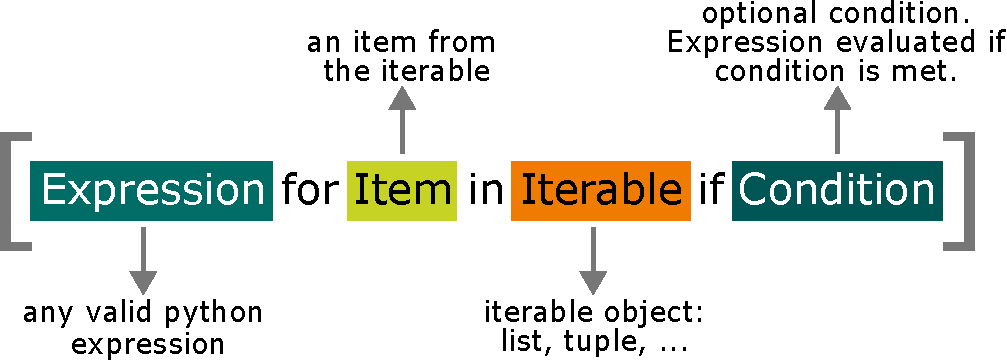
\includegraphics[width=0.6\linewidth]{img/list_comprehension.pdf}
\end{figure}

with list comprehension:
\begin{lstlisting}
squared_numbers = [i**2 for i in range(10) if i % 2 == 0]
\end{lstlisting}
\end{frame}


\begin{frame}[fragile]{while loops}
\begin{itemize}
    \item Executes a set of statement as long as a condition is true.
    \item \code|else| statement gets executed when the condition is no longer true.
    \item Works with \code|break| and \code|continue| statements.
    \item Can be thought of as a fusion between if clauses and for loops.
\end{itemize}
\begin{lstlisting}
i = 0
while i < 6:
  print(i)
  i += 1
else:
  print("i is no longer less than 6")
\end{lstlisting}
\alert{Make sure that the exit condition will (eventually) happen!}
\end{frame}


\section{Functions and Classes}
\begin{frame}[fragile]{Defining functions}
\begin{itemize}
\small
    \item Functions are short modules that accomplish a specific task.
    \item They are defined with the \code|def| keyword and the parameters in the parantheses.
    \item Functions always return something. If undefined the function returns \code|None|.
\end{itemize}

\begin{lstlisting}
def fib(n, a=0, b=1): 
    """Print a Fibonacci series up to n."""
    result = []
    while a < n:
        result.append(a)        
        a, b = b, a+b
    return result
\end{lstlisting}

\begin{lstlisting}
>>> fib(500)    # == fib(n=500, a=0, b=1) or fib(500,0,1)
Out: [0, 1, 1, 2, 3, 5, 8, 13, 21, 34, 55, 89, 144, 233, 377] 
\end{lstlisting}
\end{frame}

\begin{frame}[fragile]{Functions - tips}
    \begin{itemize}
        \item Default values for arguments can be specified:
        \begin{lstlisting}
def square_x(x, y = 2):
    return x ** y
\end{lstlisting}
    \item Variables defined inside a function are \alert{only valid within that function}.
    \item To use variables from the global namespace use \code|global|. Use it only if \alert{absolutely necessary!}
        \end{itemize}

\begin{columns}
 \column{0.5\linewidth}
 \begin{lstlisting}
def f():
    global x
    x = 40
    print(x)
\end{lstlisting}
\column{0.4\linewidth}

\begin{lstlisting}
>>> x = 20
>>> f()
Out: 40
>>> x
Out: 40
\end{lstlisting}
\end{columns}

\end{frame}

\begin{frame}[fragile]{Classes}

\begin{itemize}
    \item Classes are abstract blueprints from which objects are created.
    \item Instances are realizations of the abstract blueprint and have actual values.
    \item Classes often bundle data and functions together.
    \item New instances of a class can have different properties.
\end{itemize}
Simple class definition:

\begin{lstlisting}
class MyClass:
  x = 5

\end{lstlisting}
\end{frame}

\begin{frame}[fragile]{Class example}

Defining a new class \code|Dog|:
\begin{lstlisting}
class Dog:
    kind = 'canine'         # class variable shared by all instances

    def __init__(self, name, breed, age):
        self.name = name    # instance variable unique to each instance
        self.breed = breed
        self.age = age
        self.tricks = []
        
    def describe(self): # class method
        print(self.name, "is a(n)", self.breed, "and", self.age, "years old.")

    def add_trick(self, trick):
        self.tricks.append(trick) # We can change instance variables.
\end{lstlisting}
\end{frame}

\begin{frame}[fragile]{Class instances}
    
Create a new instance of this class and call its method function:
\begin{lstlisting}
>>> d = Dog(name = "Rex", breed = "German Shepherd", age = 4)
>>> d.kind
Out: 'canine'
>>> d.describe()
Out: "Rex is a German Shepherd and 4 years old."
\end{lstlisting}
We can create a second instance:

\begin{lstlisting}
>>> d2 = Dog(name = "Laika", breed = "unknown breed", age = 3)
>>> d2.add_trick("roll over")
>>> d2.add_trick("fly to space")
>>> d2.tricks
Out: ['roll over', 'fly to space']
>>> d.tricks
Out: [] 
\end{lstlisting}

\end{frame}

\begin{frame}[fragile]{Class inheritance}
\begin{itemize}
    \item Classes can inherit properties from a parent Class
    \item The parent class can also be from an external library.
    \item Derived classes may override methods of their base classes.
\end{itemize}
\begin{lstlisting}
class DerivedClassName(BaseClassName):
    pass
\end{lstlisting}
\begin{itemize}
    \item Check inheritance with \code|isinstance()|:
\end{itemize}
\begin{lstlisting}
>>> isinstance(d, Dog)
Out: True
\end{lstlisting}
\end{frame}



\section{Libraries}

\begin{frame}[fragile]{What are libraries?}

\begin{itemize}
    \item A python library is a collection of related modules or functions.
    \item Libraries allow us to reuse code for different projects.

    \item The python standard library consists of ~200 modules for basic system functionality (e.g. I/O).
    \begin{itemize}
        \item The python standard library comes pre-installed with python. 
        \item \url{https://docs.python.org/3/library/index.html}
    \end{itemize}

    \item Making a library out of your own code is easy!

\end{itemize}
    
\end{frame}


\begin{frame}{Useful libraries - General}
    For general use:
    \begin{itemize}
        \item \textbf{os:} For accessing the operating system.
        \item \textbf{Numpy:} Numeric Python. For working with Matrices.
        \item \textbf{Pandas:} For working and manipulating with tabulated data.
        \item \textbf{SciPy:} Scientific Python. Contains functions for common scientific computations.
        \item \textbf{PyTorch:} Machine Learning, Neural Nets, ...
        \item \textbf{Matplotlib:} For plotting.
        \item \textbf{Seaborn:} Built on Matplotlib but easier to use, esp. with Pandas.
    \end{itemize}
\end{frame}

\begin{frame}{Useful libraries}

    Image manipulation:
    \begin{itemize}
        \item \textbf{Python Imaging Library (PIL):} General image handling.
        \item \textbf{OpenCV/cv2:} Computer vision library with many useful functions (e.g. edge detection etc.).
        \item \textbf{PyTorch:} (again) machine learning tools for images.
    \end{itemize}
\end{frame}

\begin{frame}[fragile]{Pandas}
\begin{itemize}
    \item Provides the 2D \code|DataFrame| and 1D \code|Series| classes for handling data.
\end{itemize}

\begin{lstlisting}
import numpy as np
import pandas as pd

df = pd.DataFrame(np.random.randn(6, 4), 
                  index = ["R1", "R2", "R3", "R4", "R5", "R6"],
                  columns=["C1", "C2", "C3", "C4"])

\end{lstlisting}
\begin{lstlisting}
>>> df
\end{lstlisting}
\begin{table}[]
\tiny
    \begin{tabular}{cSSSS}
\toprule
 & {C1}  &   {C2}  &   {C3}  & {C4} \\
\midrule
R1  &   -0.297058 &  -1.201026 &  0.270988  &  -0.213413 \\
R2  &   0.090518  &  0.038817  &  -0.306152 &  -0.415315 \\
R3  &  0.700081   &  0.476054  &  0.558491  &  0.358557 \\
R4  &  0.535402   & -0.094973  & 2.247575   & -0.210451 \\
R5  &   -1.407642 &  0.135530  & 0.062964   &  0.474207 \\
R6  &   -1.111652 &  0.877221  &  0.427484  &  0.360299 \\
\bottomrule
    \end{tabular}

\end{table}
\end{frame}

\begin{frame}[fragile]{Viewing data}

\begin{itemize}
    \item Use \code|df.head()| and \code|df.tail()| to view the top and bottom rows of the data frame.
    \item Use \lstinline{df.to_numpy()} to convert back to numpy array.
    \item \code|df.index| and \code{df.columns} return the row and column names.
    \item Slicing can be done either with \code{df.iloc} or by label \code{df.loc}.
\end{itemize}

\begin{lstlisting}
>>> df.iloc[0:2, 0:2]
>>> df.loc["R1":"R2", ["C1", "C2"]]
\end{lstlisting}

\end{frame}

\begin{frame}[fragile]{Reading in text files}
\begin{itemize}
    \item There are many ways of reading in a text file in python.
    \item The \code{with} statement makes sure all files are closed in the end.
    \item For unstructured files one can use the following:
\end{itemize}

\begin{lstlisting}
# read from a file without with.
file = open("lorem.txt", "r+")
lines = file.read().splitlines()
file.close()

# write to a file with "with"
with open("newfile.txt", "w") as file2:
    newline = "text to add to file"
    file2.write(newline)
\end{lstlisting}
\end{frame}

\begin{frame}[fragile]{Reading in .csv files}
\begin{itemize}
    \item For .csv files either use numpy or pandas.
    \item Pandas \code{read_csv} creates a data frame, whereas \code{genfromtxt} creates a numpy array.
\end{itemize}
\vspace{0.5cm}
\begin{columns}

\column{0.4\linewidth}
\textbf{Pandas:}
\begin{lstlisting}
import pandas as pd
df = pd.read_csv('iris.csv', 
                 sep=',')
\end{lstlisting}

\column{0.4\linewidth}
\textbf{Numpy:}
\begin{lstlisting}
import numpy as np
mat = np.genfromtxt('iris.csv', 
                    delimiter=',',
                    skip_header = 1,
                    usecols = range(4))
\end{lstlisting}
\end{columns}

\begin{alertblock}{Note}
For data of mixed types use pandas! Numpy expects all data to be of the same type!
\end{alertblock}
\end{frame}


\begin{frame}[fragile]{Writing .csv files}
\begin{itemize}
    \item Writing .csv files can be done with both packages again.
    \item Pandas \code{to_csv} or numpy's \code{savetxt}.
\end{itemize}
\vspace{0.5cm}
\begin{columns}

\column{0.4\linewidth}
\textbf{Pandas:}
\begin{lstlisting}
# if you want to keep 
# rownames: index=True
df.to_csv("pd_iris.csv", 
          sep=',',
          index=False)
\end{lstlisting}

\column{0.4\linewidth}
\textbf{Numpy:}
\begin{lstlisting}
np.savetxt("np_iris.csv", 
           mat, 
           delimiter=",")
\end{lstlisting}
\end{columns}

\end{frame}

\begin{frame}[fragile]{Plotting with seaborn}
\begin{itemize}
    \item The Seaborn library allows for easy plotting.
    \item Takes pandas data frame as input.
\end{itemize}

\begin{columns}
\column{.4\linewidth}
    
\begin{lstlisting}
import seaborn as sns
sns.kdeplot(data=df)
\end{lstlisting}

\column{.5\linewidth}
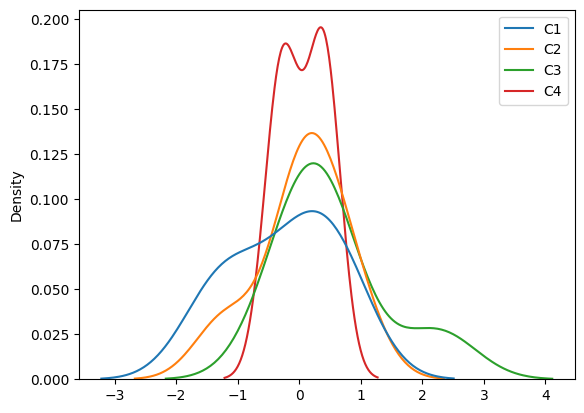
\includegraphics[width = \linewidth]{img/kdeplot.png}

\end{columns}

\end{frame}

\begin{frame}{Python Cookbook}

\begin{figure}
    \centering
    \includegraphicscopyright[height = .75\textheight]{img/cookbook.png}{Beazley, D. and Jones, B.K., 2013. Python cookbook: Recipes for mastering Python 3. " O'Reilly Media, Inc.".}
    \label{fig:enter-label}
\end{figure}

\end{frame}

\begin{frame}[fragile]{Conda environments}
\begin{itemize}
    \item Often certain libraries require certain python versions and/or versions of other libraries.
    \item These requirements can be mutually exclusive between libraries.
    \item How to manage different versions?
    \item \alert{Solution:} Conda (\url{www.conda.io}) is a package and environment management system.
    \item It allows to install different versions of python in parallel and keep different packages for different tasks.
    
\end{itemize}
\end{frame}




\section{Examples}


\begin{frame}[fragile]{The Value(s) of A Picture}
\begin{figure}
    \centering
		\includegraphicscopyright[height=3.5cm]{"img/starry_night.jpg"}{\small
  https://tinyurl.com/starrynightjpg}
\end{figure}
\begin{lstlisting}
import matplotlib.pyplot as plt
import numpy as np

img = plt.imread('starry_night.jpg')
img.shape # Order of channels: RGB
\end{lstlisting}
\end{frame}

\begin{frame}[fragile]{Plotting a single color channel}

\alert{Task:} Plot the blue channel (or any other channel) of the picture in the respective color.
\vspace{-0.5cm}
\begin{columns}
 \column{0.5\linewidth}
\begin{lstlisting}
# Decide on channel to plot
...
# Plot picture. 
# use cmap to set color!
...
\end{lstlisting}
 \column{0.4\linewidth}
 \centering
 \includegraphicscopyright[width = \linewidth]{img/blue_channel.png}{}
\end{columns}\vspace{-0.5cm}
\begin{alertblock}{Remember:}
You can use \code{imshow} from \texttt{matplotlib.pyplot} to plot an array
\end{alertblock}
\end{frame}


\begin{frame}[fragile]{Plotting a single color channel}
\begin{columns}
 \column{0.5\linewidth}
\begin{lstlisting}
import matplotlib.pyplot as plt

# Show just blue channel
plt.imshow(img[:,:,2], cmap='Blues')
plt.show()
\end{lstlisting}
 \column{0.4\linewidth}
 \centering
 \includegraphicscopyright[width = \linewidth]{img/blue_channel.png}{}
\end{columns}\vspace{-0.5cm}
\begin{alertblock}{Note:}
\texttt{cmap} controls the output colors: \url{https://matplotlib.org/stable/users/explain/colors/colormaps.html}
\end{alertblock}
\end{frame}

\begin{frame}[fragile]{Cropping}

\begin{columns}
 \column{0.5\linewidth}
 \begin{itemize}
    \item To crop just specify the indices of the matrix.
\end{itemize}
\begin{lstlisting}
# slice and plot image
...
\end{lstlisting}
 \column{0.4\linewidth}
 \centering
 \includegraphicscopyright[width = 4cm]{img/crop.png}{}
\end{columns}
\end{frame}



\begin{frame}[fragile]{Cropping}

\begin{columns}
 \column{0.5\linewidth}
 \begin{itemize}
    \item To crop just specify the indices of the matrix.
\end{itemize}
\begin{lstlisting}
cropped = img[200:, 200:270, :]
plt.imshow(cropped)
\end{lstlisting}
 \column{0.4\linewidth}
 \centering
 \includegraphicscopyright[width = 4cm]{img/crop.png}{}
\end{columns}
\end{frame}


\begin{frame}{Example: Edge detection}

\begin{columns}
\column{0.6\linewidth}
\begin{itemize}
        \small
        \item Edges can be found through the image derivatives $I_x$ and $I_y$ along the x and y axis .
        \item They describe how image intensity changes over the image.
        \item In most cases they are approximated with convolutions.
        \item A popular choice is the Sobel filter:
        {\footnotesize \begin{equation*}
D_x = 
\begin{bmatrix}
-1 & 0 & 1\\
-2 & 0 & 2 \\
-1 & 0 & 1
\end{bmatrix}, 
D_y = 
\begin{bmatrix}
-1 & -2 & -1\\
0 & 0 & 0 \\
1 & 2 & 1
\end{bmatrix}
\end{equation*}}
        % 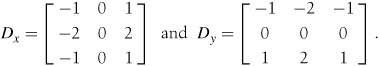
\includegraphics[width = 4cm]{img/sobel.jpg}
    \item The magnitude of the image gradient $\nabla I = [I_x, I_y]^T$ is just its length: 
$|\nabla I| = \sqrt{I_{x}^{2}, I_{y}^{2}}$.
\end{itemize}
\column{0.4\linewidth}
\includegraphicscopyright[width = \linewidth]{img/conv.png}{\center \href{https://i.stack.imgur.com/YDusp.png}{https://i.stack.imgur.com/YDusp.png}}

 \end{columns}
\end{frame}


\begin{frame}[fragile]{Convert to grayscale}

\textbf{Step 1:} Convert to grayscale image:
\begin{lstlisting}
img = plt.imread('starry_night.jpg')

# Convert to grayscale:
# Red*0.2989 + Green*0.5870 + Blue*0.1140
# Honestly, no clue why these numbers.
...
# Plot
...
\end{lstlisting}
\begin{alertblock}{Tip}
If a is an N-D array and b is a 1-D array, \texttt{np.dot(a,b)} is a sum product over the last axis of a and b. \textbf{What about \texttt{np.matmul}}?\end{alertblock}
\end{frame}

\begin{frame}[fragile]{Convert to grayscale}

\textbf{Step 1:} Convert to grayscale image:
\begin{lstlisting}
img = plt.imread('starry_night.jpg')

# np.matmul would give the same result! Why?
def rgb2gray(rgb):
    return np.dot(rgb[...,:3], [0.2989, 0.5870, 0.1140])

gray_img = rgb2gray(img)

plt.imshow(gray_img, cmap='gray')
plt.show()
\end{lstlisting}
\end{frame}

\begin{frame}[fragile]{Convolution}
\textbf{Step 2:} Convolution with Sobel Filter.
\begin{lstlisting}
# Make array for Sobel filter Dx
...
# Make array for Sobel filter Dy
...
# Convolve image with filters
# Consider image size when convolving them.
...
# Calculate magnitude
...
\end{lstlisting}
\begin{alertblock}{Tip}
You can use the \code{convolve} function from \texttt{scipy.signal}!
\end{alertblock}
\end{frame}


\begin{frame}[fragile]{Convolution}
\textbf{Step 2:} Convolution with Sobel Filter.
\begin{lstlisting}
from scipy.signal import convolve

sobel_x= np.array([[-1, 0, 1], 
                   [-2, 0, 2],
                   [-1, 0, 1]])
                   
sobel_y= np.array([[-1, -2, -1], 
                   [ 0,  0,  0], 
                   [ 1,  2,  1]])

Ix = convolve(gray_img, sobel_x, mode='same')
Iy = convolve(gray_img, sobel_y, mode='same')

grad_magnitude = np.sqrt(np.square(Ix) + np.square(Iy))
\end{lstlisting}

\end{frame}

\begin{frame}[fragile]{Example: Edge detection - Results}
\textbf{Step 3:} Plot results.
\begin{lstlisting}
plt.imshow(grad_magnitude, cmap='gray')
plt.show()
\end{lstlisting}
\begin{figure}
    \centering
    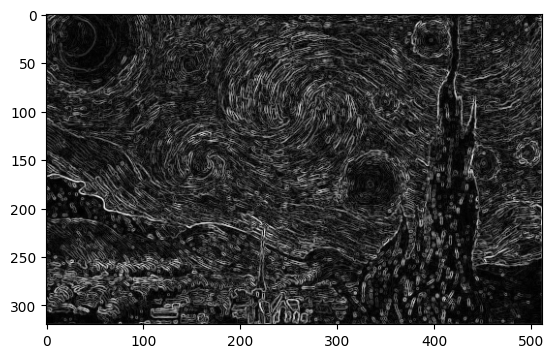
\includegraphics[width = 7 cm]{img/grad_magnitude.png}
    % \caption{\small Starry Night image gradient.}
    \label{fig:enter-label}
\end{figure}
\end{frame}

\begin{frame}[fragile]{Pig tissue}
\begin{columns}
    \column{0.5\linewidth}

\begin{lstlisting}
import cv2
img = cv2.imread('pig_tissue.tif')
# Reduce picture size.
img = cv2.resize(img, None, fx=0.5, fy=0.5)
# convert BGR to RGB colors
img = cv2.cvtColor(img, cv2.COLOR_BGR2RGB)
# same as the more cryptic img = img[...,::-1]

plt.imshow(img)
\end{lstlisting}
    
\column{0.4\linewidth}
\begin{figure}
    \centering
    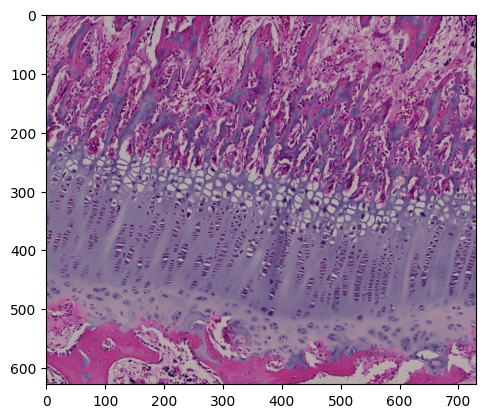
\includegraphics[width = 1\linewidth]{img/pig_python.png}
\end{figure}
\end{columns}
\alert{Task:} Rotate image around the center by 8° and crop in by 120\,\%.
\end{frame}

\begin{frame}[fragile]{Rotate image}
\alert{Task:} Rotate image around the center by 8° and crop in by 120\,\%.
\vspace{-0.2cm}
\begin{columns}
    \column{0.6\linewidth}
    \begin{lstlisting}
# find center of image
...
# make rotation matrix, f(center, degrees, scale)
...
# rotate image
...
# plot
...
\end{lstlisting}
\column{0.35\linewidth}
\begin{figure}
    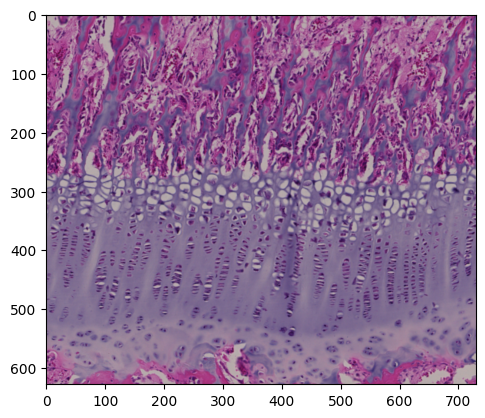
\includegraphics[width = 1\linewidth,left]{img/pig_rotated.png}
\end{figure}
\end{columns}\vspace{-0cm}
\begin{alertblock}{Tip}
You can use \texttt{cv2.getRotationMatrix2D()} and \texttt{cv2.warpAffine()}.
\end{alertblock}
\end{frame}


\begin{frame}[fragile]{Rotate image}
\begin{columns}
    \column{0.6\linewidth}
    \begin{lstlisting}
# find center of image
height, width = img.shape[:2]
centerX, centerY = (width // 2, height // 2)

# rotation matrix, f(center, degrees, scale)
M = cv2.getRotationMatrix2D((centerX, centerY), 8, 1.2)

# rotate image
rotated = cv2.warpAffine(img, M, (width, height)) 
plt.imshow(rotated)
\end{lstlisting}
\column{0.35\linewidth}
\begin{figure}
    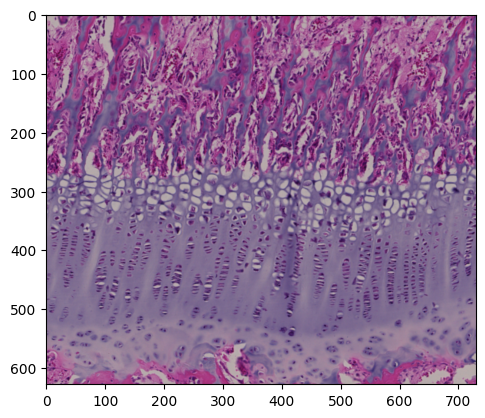
\includegraphics[width = 1\linewidth,left]{img/pig_rotated.png}
\end{figure}
\end{columns}

\end{frame}

\begin{frame}[fragile]{Mean RGB}
Calculate row-wise mean over each channel seperately:
\begin{lstlisting}
# Calc. row-wise mean
...
# Convert to pandas data frame
...
# Optional: pivot from wide to long format.
...
\end{lstlisting}
\begin{alertblock}{Tip}
Checkout the documentation to \texttt{pandas.DataFrame}!
\end{alertblock}
\end{frame}


\begin{frame}[fragile]{Mean RGB}
Calculate row-wise mean over each channel seperately:
\begin{lstlisting}
row_mean = rotated.mean(axis=1) # row-wise mean

# Convert to pandas data frame
rgb = pd.DataFrame(row_mean,
                    columns = ["Red", "Green", "Blue"])

rgb["row"] = range(row_mean.shape[0])
rgb.set_index("row")
rgb_long = pd.melt(rgb, id_vars = "row", var_name="channel", value_vars=["Red", "Green", "Blue"])

\end{lstlisting}
\end{frame}


\begin{frame}[fragile]{RGB lineplot}

Plot RGB channels over the rows:
\begin{columns}
    \column{0.4\linewidth}
\begin{lstlisting}
# Optional: Pick custom colors.
...
# Use seaborn to plot d
# plot pandas dataframe.
...
\end{lstlisting}
\column{0.5\linewidth}
\begin{figure}
    \centering
    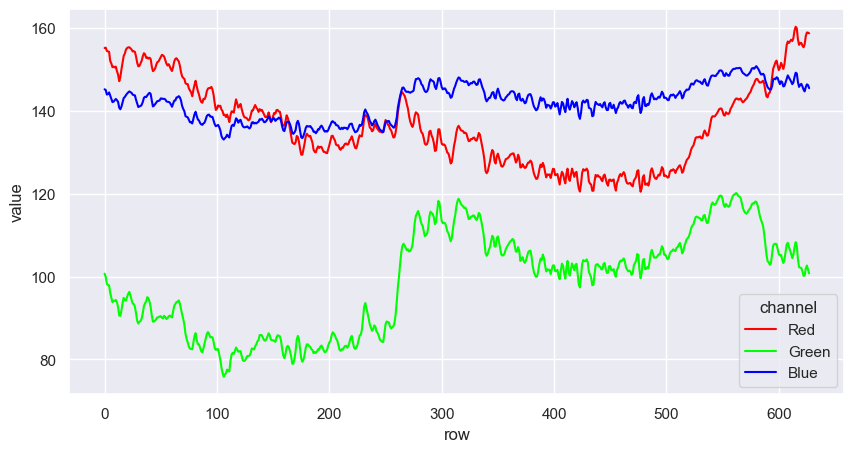
\includegraphics[width = 1\linewidth]{img/rgb_lines.png}
\end{figure}
\end{columns}
\begin{exampleblock} {Note}
\small
Instead of seaborn and pandas one could use matplotlib to directly plot the numpy array. Because it is arguably much more cryptic and difficult to learn this is skipped here.
\end{exampleblock}
\end{frame}



\begin{frame}[fragile]{RGB lineplot}

Plot RGB channels over the rows:
\begin{lstlisting}
colors = ["#FF0000", "#00FF00", "#0000FF"]
sns.lineplot(rgb_long, x="row", y = "value", hue = "channel", palette = colors)
\end{lstlisting}
\begin{figure}
    \centering
    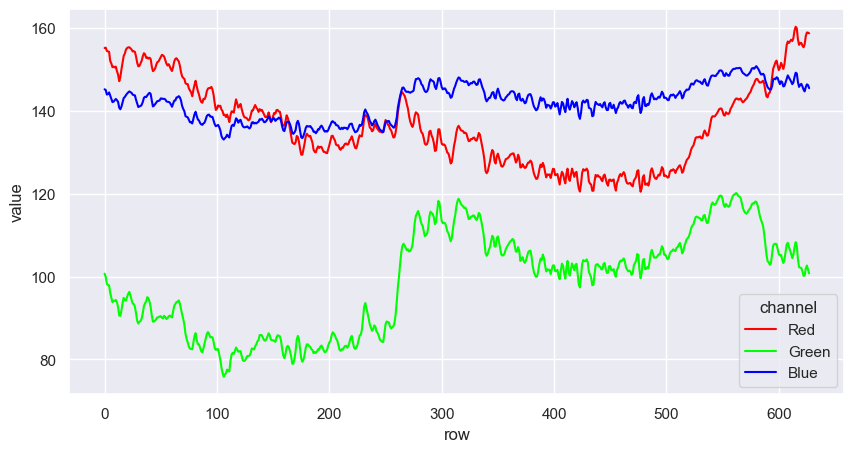
\includegraphics[width = 0.6\linewidth]{img/rgb_lines.png}
\end{figure}
\end{frame}



\setbeamertemplate{caption}{\raggedright\insertcaption\par}
\begin{frame}{Example solutions}
\begin{columns}
    \column{0.5\linewidth}
    \begin{itemize}
    \item Open Jupyter Notebook from Link
    \item File > "Save a Copy in Drive"
    \item Execute Cells with "Ctrl + Enter" or "Shift + Enter"
\end{itemize}
    \column{0.4\linewidth}
    \begin{figure}
    \centering
    
\includegraphics[width = 0.7\linewidth]{img/example_qr.png}
    \caption{\alert{\url{www.tinyurl.com/mr3x2se6}}}
\end{figure}
\end{columns}

\end{frame}
\setbeamertemplate{caption}[default]




\end{document}






